\section{Создание приложения}

\subsection{Состав и Характеристики файлов проекта}
\begin{table}[!h]
    \centering
    \begin{tabular}{p{0.35\linewidth} | p{0.6\linewidth}|}
        \hline
        \multicolumn{2}{|l|}{Заголовочные файлы} \\ \hline
        \multicolumn{1}{|l|}{WiimoteHid.hpp} & Основной заголовочный файл проекта, подключающий внешние заголовочные файлы и необходимый для работы с библиотекой.
        Также в нём происходит объявление функций библиотеки. \\ \hline
        \multicolumn{2}{|l|}{Файлы исходного кода} \\ \hline
        \multicolumn{1}{|l|}{WiimoteHid.сpp} & Содержит реализацию функций объявленных в WiimoteHid.hpp \\ \hline
        \multicolumn{1}{|l|}{lib.rs} & Является абстракцией над библиотекой для предоставления упрощённого интерфейса взаимодействия с геймпадом Wiimote \\ \hline
        \multicolumn{2}{|l|}{Вспомогательные файлы} \\ \hline
        \multicolumn{1}{|l|}{bindings.rs} & Сгенерированные из WiimoteHid.hpp с помощью инструмента bindgen.
        Необходим для компиляции lib.rs. \\ \hline
    \end{tabular}
    \caption{\label{tab:table-name}Описание файлов проекта}
\end{table}
\subsection{Стандартные классы и функции приложения}
\begin{tabularx}{\linewidth}{|X|X|X|}
    \hline
        Название & Назначение & Параметры \\ \hline
        BluetoothFindFirstRadio & Получение handle'а к bluetooth модулю.
        & Принимает указатель на структуру с параметрами, по которым будет вестись поиск, а так же указатель на handle. \\ \hline
        BluetoothFindNextRadio & Возвращает handle к следующему bluetooth модулю, если тот имеется.
        & Принимает handle на предыдущий модуль, и handle куда будет записан новый в случае нахождения. \\ \hline
        BluetoothGetRadioInfo & Получение данных таких, как адрес, имя, класс устройства и информации производителя, о bluetooth модуле.
        & Принимает структуру, в которую будет записана информация, и handle к модулю. \\ \hline
        BluetoothFindFirstDevice & Получение handle'а первого найденного устройства в зоне действия bluetooth модуля.
        & Принимает структуру, куда будет записана информация о найденном устройстве, и параметрами, по которым будет вестись поиск. \\ \hline
        BluetoothFindNextDevice & Получение handle'а следующего найденного устройства.
        & Принимает структуру, куда будет записана информация о найденном устройстве, и параметрами, по которым будет вестись поиск. \\ \hline
        CloseHandle & Закрывает(возвращает системе) handle.
        & Принимает handle, который планируется закрыть. \\ \hline
        wcscmp & Возвращает разницу между переданными строками.
        & Принимает два указателя на wchar\_t \\ \hline
        BluetoothRemoveDevice & Удаляет устройство из списка прежде подключённых в операционной.
        & Принимает адрес устройства, которое надо удалить. \\ \hline
        BluetoothSetServiceState & Устанавливает состояние bluetooth сервиса Windows, например для указания сопряжения с устройством.
        & Принимает handle к bluetooth модулю, информации об устройстве, ID сервиса, через который будет происходить работа, устанавливаемое состояние. \\ \hline
        HidD\_GetHidGuid & Получение id для HID сервиса.
        & Принимает ссылку на переменную куда будет записан id. \\ \hline
        SetupDiGetClassDevs & Функция возвращает дескриптор набора информации об устройстве, который содержит запрошенные элементы информации.
        & Принимает указатель на устройство, счётчик, handle к окну и флаги. \\ \hline
        SetupDiEnumDeviceInterfaces & Функция SetupDiEnumDeviceInterfaces перечисляет интерфейсы устройств, которые содержатся в наборе информации об устройстве.
        & Принимает DeviceInfoSet, DeviceInfoData, ID устройства, индекс, переменную куда будут записаны данные. \\ \hline
        HidD\_GetAttributes & Возвращает атрибуты переданного устройства.
        & Получает handle устройства, и ссылку на структуру, куда будут записаны дынные. \\ \hline
        CreateEvent & Служит для создания объекта события.
        & Получает указатель на структуру SECURITY\_ATTRIBUTES, булевую переменную устанавливающую автоматический или ручной перезапуск, булевое начальное состояние, имя события. \\ \hline
        ResetEvent & Перезапускает событие.
        & Получает ссылку на событие. \\ \hline
        WriteFile & Записывает данные в указанный файл или устройство ввода/вывода (I/O).
        & Получает handle куда будет производиться запись, указатель на записываемые данные, количество записываемых байтов, ссылка на переменную куда будет записано количество отправленных байтов, указатель на переменную, которая содержит информацию, используемую при асинхронном (или перекрывающемся) вводе и выводе. \\ \hline
        ReadFile & Считывает данные из указанного файла или устройства ввода/вывода (I/O).
        & Получает handle устройства/файла, указатель на буфер куда будут прочитаны данные, количество считываемых байтов, ссылка на переменную куда будет записано количество полученных байтов, указатель на переменную, которая содержит информацию, используемую при асинхронном (или перекрывающемся) вводе и выводе. \\ \hline
        WaitForSingleObject & Ожидает событие в течение указанного времени.
        & Получает указатель на событие. \\ \hline
        CancelIo & Отменяет ожидания ввода и вывода для устройства/файла.
        & Получает дескриптор устройства. \\ \hline
        GetOverlappedResult & Извлекает результаты перекрывающейся/асинхронной операции с указанным файлом, или устройством, или именованным каналом.
        & Получает дескриптор устройства, ссылку на OVERLAPPED, ссылку на переменную куда будет записано количество прочитанных байтов, время ожидания. \\ \hline
        \caption{\label{tab:table} Таблица с описанием стандартных использованных функций}
\end{tabularx}
\subsection{Пользовательские структуры в приложении}
\subsubsection{struct wiimote\_hid}
\quad Необходима для хранения:\\
\quad Hid дескриптора, через который происходит обращение к устройству\\
\quad Переменной типа OVERLAPPED, предназначенной синхронизации с потоками ввода и вывода\\
\quad Буфера, используемого при чтении и записи.\\
Через данную структуру происходит получение и отправка данных.
Для этого содержит методы чтения и записи.

\subsubsection{struct bluetooth\_device}
\quad В данной структуре хранится HANDLE к bluetooth модулю и BLUETOOTH\_DEVICE\_INFO\_STRUCT, с помощью которого происходит обращение к устройству.


\subsection{Пользовательские функции в приложении}
\subsubsection{wiimote\_hid::write()}
\quad Предназначена для записи данных из буфера структуры wiimote\_hid.

\subsubsection{wiimote\_hid::read()}
\quad Предназначена для записи данных в буфер структуры wiimote\_hid.
Возвращает количество прочитанных байтов.

\subsubsection{GetWiimoteHid()}
\quad Производит поиск геймпада среди подключённых hid устройств и при нахождении устанавливает с ним соединение.\\
\quad Возвращает структуру wiimote\_hid.

\subsubsection{void ProcessWiimotes(bool new\_scan, const T \&callback = nullptr)}
\quad Производит поиск bluetooth устройств.
При нахождении такого производит вызов callback функцию, устанавливающую соединение.

\subsubsection{bool AttachWiimote(HANDLE hRadio, const BLUETOOTH\_RADIO\_INFO \&radio\_info, BLUETOOTH\_DEVICE\_INFO\_STRUCT \&deviceInfo)}
\quad Устанавливает соединение с геймпадом.

\subsubsection{bool ForgetWiimote(BLUETOOTH\_DEVICE\_INFO\_STRUCT \&deviceInfo)}
\quad Производит удаление удаление устройства из списка операционной системы с ранее подключёнными устройствами.

\subsubsection{void wiimoteDisconnect(bluetooth\_device *bluetoothDevice)}
\quad Разрывает bluetooth соединение с геймпадом.

\subsubsection{bluetooth\_device *FindConnectWiimoteBLE()}
\quad Производит цикл поиска и подключения к устройству и возвращает структуру с дескриптором к bluetooth модулю и информацией о bluetooth-устройстве.
\newcommand{\centered}[1]{\begin{tabular}{l} #1 \end{tabular}}
\subsection{Пользовательские функции в приложении}
\begin{tabularx}{\linewidth}{|X|X|}
    \hline
    wiimote\_hid::write& Предназначена для записи данных из буфера структуры wiimote\_hid.\\\hline

    wiimote\_hid::read& Предназначена для записи данных в буфер структуры wiimote\_hid.Возвращает количество прочитанных байтов.\\\hline

    GetWiimoteHid& Производит поиск геймпада среди подключённых hid устройств и при нахождении устанавливает с ним соединение.
    Возвращает структуру wiimote\_hid.\\\hline

    void ProcessWiimotes& Производит поиск bluetooth устройств.При нахождении такого производит вызов callback функцию, устанавливающую соединение.\\\hline

    bool AttachWiimote& Устанавливает соединение с геймпадом.\\\hline

    bool ForgetWiimote& Производит удаление удаление устройства из списка операционной системы с ранее подключёнными устройствами.\\\hline

    void wiimoteDisconnect& Разрывает bluetooth соединение с геймпадом.\\\hline

    bluetooth\_device *FindConnectWiimoteBLE& Производит цикл поиска и подключения к устройству и возвращает структуру с дескриптором к bluetooth модулю и информацией о bluetooth-устройстве.\\\hline
\end{tabularx}

\subsection{Структура программы}
    \begin{center}
        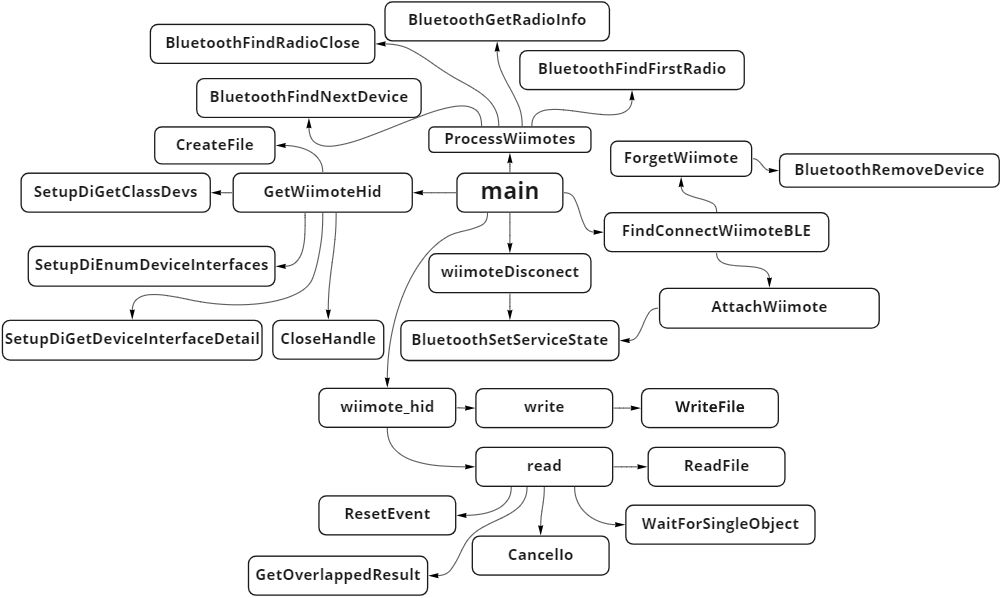
\includegraphics[width=\textwidth]{content/program_structure}

        \captionof{figure}{Структура программы}
    \end{center}

\subsection{Системные требования}
\begin{enumerate}
    \item Семейство операционных систем Windows.
    \item Наличие свободного места в размере 158кб.
    \item Bluetooth модуль.
    \item Геймпад от Nintendo Wii - Wiimote.
\end{enumerate}


